\chapter{Enabling technologies}
\label{chap:enabling}

\begin{chapterintro}

In this chapter, we describe the technologies used in this project. We start by describing the web technologies, both client and server, used when building the front end interface. Then we discuss the modules used for the conversational system, as well as ChatScript and its capabilities. Finally, we talk about the techniques used retrieving and indexing the relevant information for our system.

\end{chapterintro}

\cleardoublepage

\section{Overview}

\section{Web technologies}

% Talk about all-web movement? JavaScript & JQuery? 

% This is mostly bullshit. Rewrite it.

Known simply as ``The web'', the World Wide Web is an information system where hypertext documents are accessed via the internet. First proposed by Tim Berners Lee in 1989\cite{berners1989information}, it has grown to be used by two in five people around the world\footnote{\url{http://webfoundation.org/about/vision/history-of-the-web/}}.

The technologies used in web services can be divided in Client technologies, executed in the user's computer, and Server technologies, executed in the server side of the service. We will provide a short description of some of the technologies available for each side, focussing on those used in this project.
\subsection{Client technologies}

At its core, every web page is nothing but HTMl, CSS and JavaScript. On top of this multiple frameworks are built, allowing complex user interaction. 

\emph{\textcolor{red}{Rework this section. Talk about jQuery, the evolution of the web to dynamic pages and data, etc}}

% JS/jQuery, HTML5, CSS, etc

\subsection{Server technologies}

% HTTP Servers. Apache?

The interactions presented by the web client are the processed in the server side, usually communicating using HTTP. There are multiple applications capable of handling this interaction, known as http servers. Apache, NginX or Microsoft Windows Server\textregistered~are some of the most popular servers\footnote{\url{http://news.netcraft.com/archives/2015/05/19/may-2015-web-server-survey.html}}. 

For our service, we have used Apache\cite{apacheabout}, an Open Source HTTP-Server. First launched in 1995, it has continued development to this date, with version 2.4.12 being released on January 2015~\footnote{\url{http://httpd.apache.org/}}. It is currently developed and maintained by an open community of developers under the Apache Software Foundation, and made available in a wide variety of operating systems, including GNU/Linux and Microsoft Windows\textregistered. It features a module-based system, allowing the core functionality to be expanded by compiled modules. Some of the most popular modules include:

\begin{itemize}[topsep=0pt,itemsep=-1ex,partopsep=1ex,parsep=1ex]
 \item \textbf{mod\_php} Enabling the use php to execute server side code, this module can be found in many Apache installations, allowing the deployment of services like WordPress or Joomla.
 \item \textbf{mod\_auth\_basic} Handling basic user authentication, this module allows the server administrator to block sections of the server from being accessed by the general public.
 \item \textbf{mod\_proxy} Allows the use of Apache as a proxy, masking other services behind it.
\end{itemize}

Over the last few years, multiple other server technologies have appeared, focusing on running code to build network applications. Node.js\footnote{\url{https://nodejs.org/}} or uWSGI\footnote{\url{http://uwsgi-docs.readthedocs.org/}} are examples of this philosophy. \emph{\textcolor{red}{This wording is weird}}

\subsubsection{WSGI Servers in python}

\ac{WSGI} is a specification for simple interfaces between web servers and web applications for the python programming language. First defined in PEP 333\cite{pep0333}, and updated in PEP 3333\cite{pep3333}, it has been adopted as a standard for python web application development.

\emph{\textcolor{red}{Read the pep3333 and complete this.}}

There are multiple implementations and frameworks of WSGI for python, some of the most popular are:

\begin{itemize}
 \item \textbf{Bottle} is a simple lightweight WSGI framework, focusing on simplicity. It is distributed as a single file module, with no other dependencies than the python standard library. However, it has capabilities to handle routing, easy access to web data such as cookies and http headers, and includes a built-in server for development. It also has support for templates, both with a built-in engine, and using external modules such as mako or jinja2.
 \item \textbf{Django} is a full-fledged python web framework, offering fast and scalable services, with multiple built-in options, such as security, administration tools. It is slightly higher level than other frameworks, and emphasizes reusability of components and plugins, as well as rapid development. % complete?
 \item \textbf{Flask}, a micro web application framework, based on the jinja2 template engine, and the Werkzeug WSGI toolkit. It focuses on providing a simple interface, whilst still providing multiple features such as RESTfull request dispatching, cookies and request handling and unicode support. It also includes native support for unit testing, as well as a development server and debugger. It also supports extensions for extra functionalities.
\end{itemize}

In our application, we have chose Apache as the gateway server, using mod\_wsgi, and Flask for the application itself. \emph{\textcolor{red}{Give ``example'' apache config?}}

% Flask, django, bottle, mod_wsgi

\section{ChatBot modules}

As we have discussed in section \ref{sec:conv_agents}, there are several chatbot technologies capable of processing natural language interactions and conversation handling.

\subsection{ChatScript}
\label{subsec:chatscript}

\emph{\textcolor{red}{Rewrite this section}}

ChatScript~\cite{wilcox2013} is a Loebner-prize winning chatbot module.

It focuses matching user input in general meaning, allowing simple and very complete bots. The default language is English, and ChatScript provides built-in dictionaries and \ac{PoS} tagging for it. It also have a knowledge system based on fact triples.

\subsubsection{Basic syntax, topics and rules}

In Chatscript, rules are grouped in topics, and stored in ``.top'' files, allowing the designer to map the point of the conversation, therefore making a better response for the user. And example topic file can be found in listing~\ref{listing:exampletop}. In this example, the topic will be triggered when the user writes an input containing the words ``name'', ``here'', ``what'', or any other word specified in the system dictionaries ``emogoodbye'', ``emohello'' or ``emohowzit''. Then, it will attempt to match the user input with the patterns ``what is your name'' and ``what ~be''. If no pattern matches, it will output the gambit ``Have you been here before?''.

\begin{center} 
  \begin{lstlisting}[language={}, captionpos=b, caption=Example topic file, label=listing:exampletop]   
    topic: ~INTRODUCTIONS (~emogoodbye ~emohello ~emohowzit name here what )
    
    #!x issued only once, then erased
    t: Have you been here before?
    
    #! what is your name 
    u: ( what is your name ) 
        My name is Harry.
        
    #! what are you ?
    ?: ( what ~be )
        I am a bot. Are you also a bot?
        a: (~no)
            Oh, a human... How can I help you?
  \end{lstlisting}
\end{center}

In this simple example, we find some of ChatScript syntaxes elements. We can see responders, gambits and rejoinders, as well as the use of topics and concepts. These are part of ChatScript rules structure, but there are some more elements not shown here. A slightly more comprehensive list is as follows:
\begin{itemize}
 \item \textbf{Input matching:} The pattern can start with either ``s:'', ``?:'' or ``u:'', indicating they are supposed to respond to statements, questions or both. The parenthesis then indicate the pattern itself, which can have multiple elements:
    \subitem \emph{General words:} A simple word to look for on the sentence. ChatScript handles plurals and verb conjugations.
    \subitem \emph{Concepts:} Starting with \~ , a concept is a set of words with a common general meaning.
    \subitem \emph{Wildcards:} Allowing to match any word, or using a cardinal, can specify the number of words to match with the wildcard.
    \subitem \emph{Start and end of sentence:} Using > and <, its possible to indicate whether the pattern should match the start or the end of the sentence.
    \subitem \emph{Variables: } Starting the pattern element, whether is a wildcard, a concept or a word, using ``\_'', will store the matched word in a variable for future use, be it in the response or somewhere else.
  \item \textbf{Gambit:} Lines starting with ``t:'' indicate a gambit, that will be triggered when the bot cannot find an appropriate response.
  \item \textbf{Bot Response:} Immediately after the pattern, the following lines until the next chatscript syntax element indicate how the bot response is formed.
  \item \textbf{Variables:} Not shown in the previous example, any word starting with ``\$'' is a global variable, and can be assigned a value that will be remembered for the user. If the variable starts with ``\$\$'', the variable will be local, only lasting until the end of the current answer.
  \item \textbf{Rejoinders} Starting with single letters from ``a:'' through ``q:'' to indicate nesting depth, this indicate patterns that will trigger when the user responds to a specific bot output.
  \item \textbf{Concepts:} Sets of word with a specific meaning, when referring to a concept in a pattern, it will match if any word in the set matches the input. ChatScript includes a large set of concepts by default, but the user can define its own sets.
  \item \textbf{Topics:} rules are grouped in topics. Rules inside the topic will only be tested against the input when the input itself contains any of the words specified while defining the topic.
\end{itemize}

A more detailed approach to ChatScript rules, matching and functions can be found in its documentation\footnote{\url{http://sourceforge.net/projects/chatscript/files/}}.

\subsubsection{Deploying a bot with ChatScript}

By default, ChatScript can be run in local or server mode. Local mode allows for direct interaction from the command line, using the standard input and output to communicate with the user. This mode is specially usefull for debugging the rules when developing bots, since it gives access to debugging commands build with the system.

For production environments, ChatScript can be run in server mode, where it listens it offers a TCP interface. This interface will receive messages containing the bot name, the user name and the user input, and return the bot response for the given input.

\section{Information retrieval}

The amount of information available in the web has grown exponentially over the last years, with standards such as Linked Data helping exchange data among heterogeneous systems. However, many times these standards are not used, and so it becomes necessary to recover and convert the data into compatible formats. There are multiple frameworks capable of crawling the web and recovering the relevant pieces of information, but we will focus here in Scrappy, a framework in ruby that allows extracting information from web pages and producing RDF data, and Scrapy, a python tool that allows extracting data from websites into any format, with powerful capabilities.

% Scrappy and scrapy

\subsection{Scrappy}

Scrappy\cite{villamor13} is a ruby framework with multiple functionalities, including web and REST interface, storing the scrapped data in a RDF repository, and outputing in multiple formats. For our system, we will discuss the web scrapping and RDF output capabilities.

To recover data from a web page, Scrappy utilizes an ontology\footnote{http://www.gsi.dit.upm.es/ontologies/scraping/} to define the mapping between the web data and the semantic web resources. An example extractor can be found in listing \ref{listing:examplescrappy} will take the link to the GSI's staff page and return a foaf object with the name of each member. As seen in the extractor, it matches CSS elements in the page to semantic properties. Although not shown in this particular example, it can also use Xpath and regular expressions as selectors.

\begin{center} 
  \begin{lstlisting}[language={}, captionpos=b, caption=Example extractor, label=listing:examplescrappy]   
dc: http://purl.org/dc/elements/1.1/
rdf: http://www.w3.org/1999/02/22-rdf-syntax-ns#
sioc: http://rdfs.org/sioc/ns#
sc: http://www.gsi.dit.upm.es/ontologies/scraping.rdf#

_:gsipeople:
  rdf:type: sc:Fragment
  sc:type: foaf:Person
  sc:selector:
    *:
      rdf:type: sc:UriPatternSelector
      rdf:value: "http://www.gsi.dit.upm.es/index.php?option=com_jresearch&view=staff&layout=positions"
  sc:identifier:
    *:
      rdf:type: sc:BaseUriSelector
  sc:subfragment:
    *:
      sc:type: foaf:Person
      sc:selector:
        *:
          rdf:type: sc:CssSelector
          rdf:value: ".jrperson"
      sc:identifier:
        *:
          rdf:type: sc:CssSelector
          rdf:value: "a"
          sc:attribute: "href"
      sc:subfragment:
        *:
          sc:type: rdf:Literal
          sc:relation: foaf:givenName
          sc:selector:
            *:
              rdf:type: sc:CssSelector
              rdf:value: "a"
  \end{lstlisting}
\end{center}

An example of data generated with that extractor is shown in listing ~\ref{listing:examplerdf}. It can be seen how the elements matched in the extractor have been converted into properties. We have keep the example simple for clarity and space reasons.

\emph{\textcolor{red}{Complete this section}}

\begin{center}
  \lstinputlisting[language=XML, captionpos=b, caption=Example person extracted with Scrappy, label=listing:examplerdf]{code/enabling/person.rdf}
\end{center}

\subsection{Scrapy}

Scrapy\footnote{\url{http://scrapy.org/}} is a fast high level web crawling framework, used to extract structured data from websites. It is written in python, and by default outputs data to json, although it accepts custom exporters, giving the user the ability to export into any format it requires.

The crawlers are python classes that extend the Spider class in scrapy.

\emph{\textcolor{red}{Add example code for scrapy. Maybe something for the gsi news?}}

\section{Information indexing}

Storing and indexing information \emph{\textcolor{red}{Justify the need to use a DB to index the info?}}
% Apache Solr? 

\subsection{Apache Solr}

Apache Solr, first described in section \ref{sec:statesolr}, is an open source search platform, written in Java and built on top of Apache Lucene, an indexing an retrieval engine. It provides full text indexing and search capabilities and faceted search, as well as a web interface, and a REST-like api for queries. Figure \ref{fig:solr1} shows the query interface in the solr web administrator.

\begin{figure}[!htbp]
    \centering
    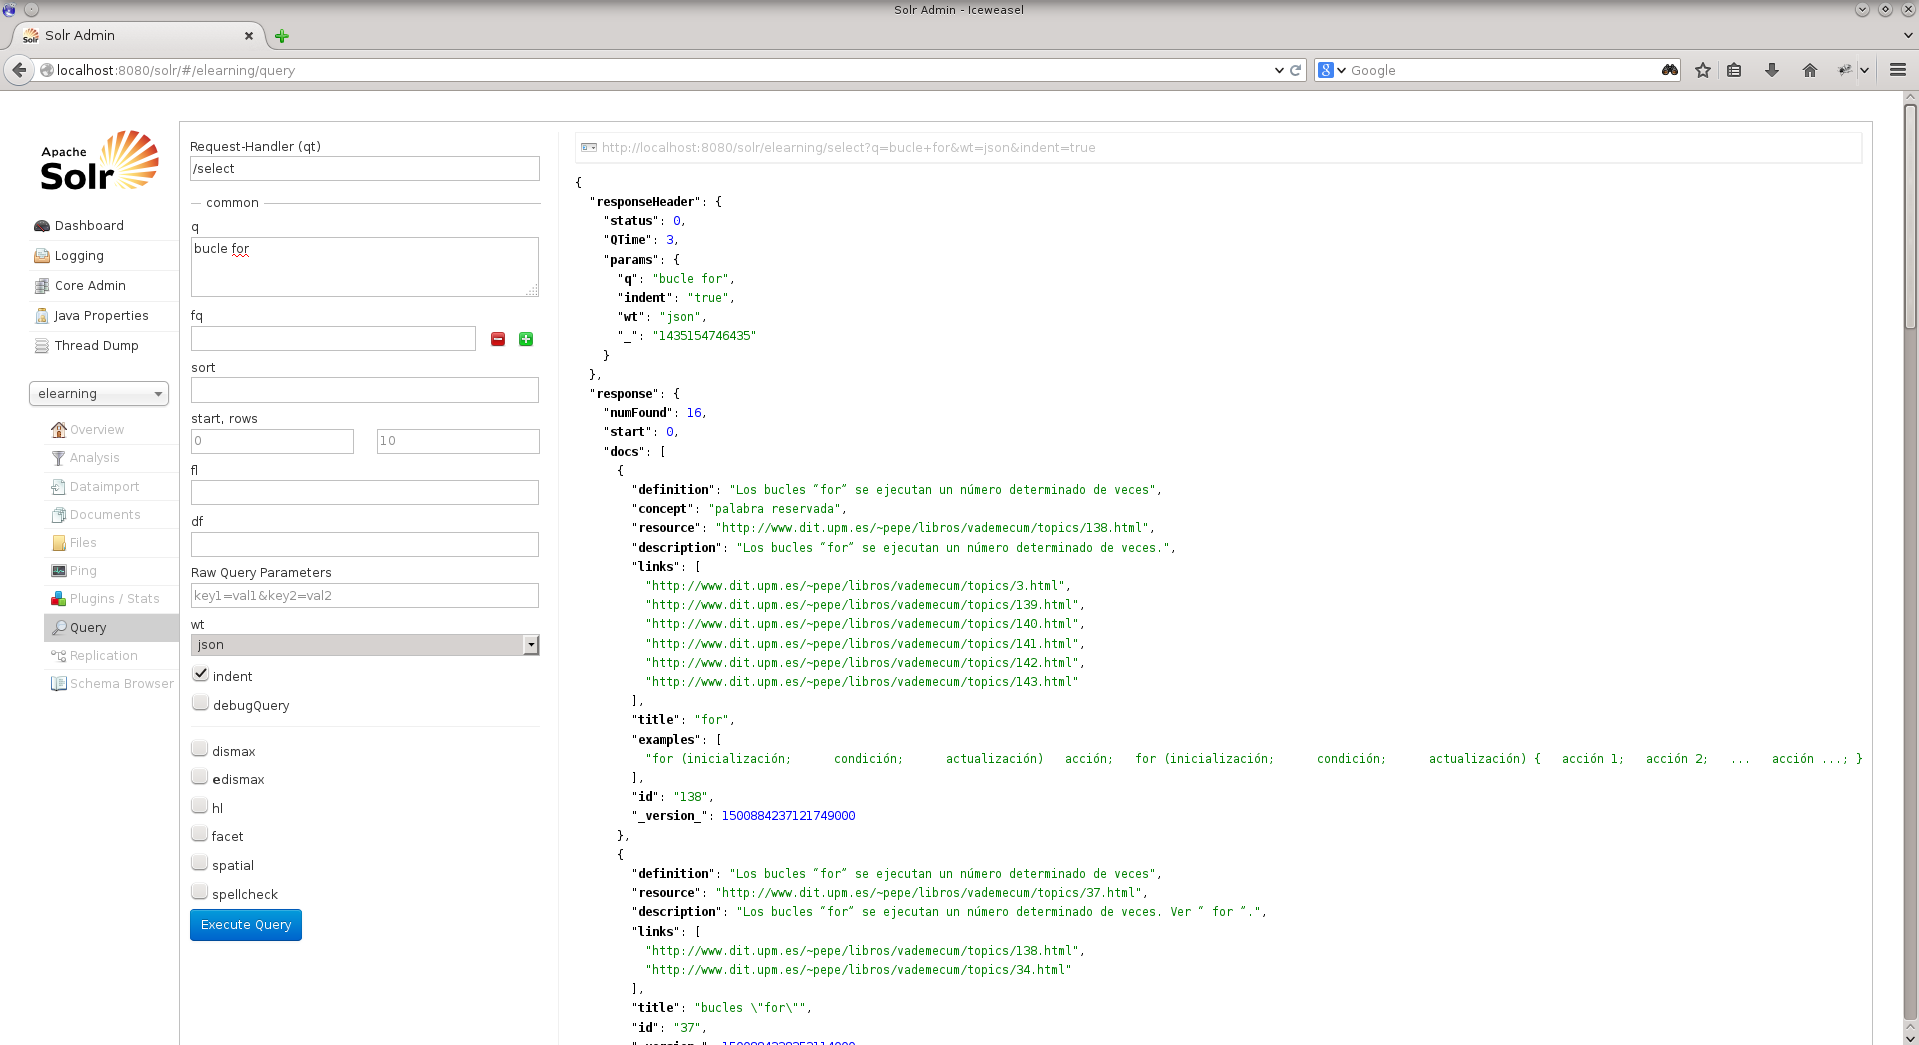
\includegraphics[width=0.9\textwidth]{img/screens/solr-interface.png}
    \caption{Web interface for Solr queries.}
    \label{fig:solr1}
\end{figure}

\emph{\textcolor{red}{Complete this section}}

% Add reference to taming text
% example query? Already done in prototype?
% example core?

\subsection{Fuseki}

% Change this paragraph! Placeholder from ruben's master thesis
Fuseki is a SPARQL server. It provides REST-style SPARQL HTTP Update, SPARQL Query, and SPARQL Update using the SPARQL protocol over HTTP. We will use a Fuseki server installation for storing our own RDF files containing geoSPARQL data.

\emph{\textcolor{red}{Complete this section}}

% Fuseki web interface
% Example rest query?